%
% Documento: Estrutura
%

\chapter{ESTRUTURA}

A estrutura de acordo com a NBR-14724, compreende três elementos: pré-textuais, tex-tuais e pós-textuais.

\begin{figure}[H]
	\vspace*{0,2cm}
    \centering
    \caption{Ilustração da estrutura}
    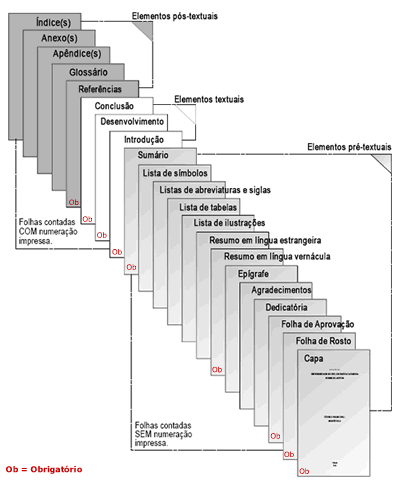
\includegraphics[width=0.6\textwidth]{./04-figuras/abnt}
    \label{fig:ilustfig2}
\end{figure}
\vspace*{-0,9cm}
{\raggedright \fonte{Disponível em: <https://www.intelligentsia.zip.net/estruturamonografia>. Acesso em: 15 ago. 2014.}}\\

Os elementos pré-textuais são compostos de estruturas
obrigatórias: Capa, Folha de ros-to, Folha de aprovação e Sumário. E estruturas opcionais: Lombada, Errata, Dedicatória, Agra-decimentos, Epígrafe, Resumo na língua vernácula, Resumo em língua estrangeira, Lista de ilustrações, Lista de abreviaturas e siglas e Lista de símbolos.

Os elementos textuais são compostos de Introdução,
Desenvolvimento e Conclusão. Os elementos pós-textuais podem é obrigatórios usar as Referências.  E são elementos opcionais: Glossário, Apêndice, Anexo e Índice.

\section{ELEMENTOS PRÉ-TEXTUAIS}

\subsection{Capa}

Elemento obrigatório, sobre o qual se imprimem as informações
indispensáveis à indica-ção do trabalho, na seguinte ordem: nome completo do aluno, título do trabalho, subtítulo se houver, cidade da instituição onde o documento deve ser apresentado, ano de depósito (data da entrega).

\subsection{Lombada}

Elemento opcional, onde as informações devem ser impressas
conforme a norma NBR 12225: nome do autor, impresso longitudinalmente e legível do alto para o pé da lombada. Esta forma possibilita a leitura quando o trabalho está no sentido horizontal, com a face voltada para cima; título do trabalho, impresso da mesma forma que o nome do autor. Elementos alfanuméri-cos de identificação, por exemplo: v. 3.

\subsection{Folha de Rosto}

O anverso da folha de rosto deve conter os elementos na seguinte
ordem: nome completo do aluno, título do trabalho, subtítulo se houver, natureza do trabalho e objetivo (grau pretendi-do), nome da instituição a que é submetido, área de concentração, nome do orientador, local da instituição onde deve ser apresentado, ano de entrega.

\subsection{Errata}

A errata consiste em uma lista das folhas e linhas em que ocorrem
erros, seguida das de-vidas correções. Deve ser inserida após a folha de rosto.

\subsection{Folha de aprovação}

Elemento obrigatório, a folha de aprovação deve conter: nome do
autor, título por exten-so, subtítulo, local e data de aprovação, nome, assinatura e instituição dos membros componen-tes da banca examinadora.

\subsection{Dedicatória}

Folha opcional, onde o aluno presta homenagem ou dedica seu trabalho.

\subsection{Agradecimentos}

Folha opcional, dirigida àqueles que contribuíram para a
elaboração do trabalho.

\subsection{Epígrafe}

Elemento opcional, onde o aluno apresenta uma citação, seguida da
indicação de autoria, relacionada com a matéria tratada no corpo do trabalho. As epígrafes também podem ser apre-sentadas nas folhas de abertura das seções primárias.

\subsection{Resumo}

Consiste na apresentação concisa dos pontos principais de um
texto. Devem ser apresen-tados, de forma clara, os objetivos, o desenvolvimento e as conclusões. Constitui-se em uma sequência de frases objetivas e não uma simples enumeração de tópicos. Deve ser seguido das palavras representativas do conteúdo do trabalho, isto é, palavras-chave e/ou descritores.

\subsection{Abstract}

Consiste em uma versão do resumo em idioma de divulgação
internacional. Deve ser se-guido das palavras representativas do conteúdo do trabalho, isto é, palavras-chave e/ou uniter-mos, na língua.

\subsection{Lista de ilustrações}

As ilustrações (figuras, quadros, tabelas, gráficos) devem ser
numeradas na ordem em que aparecem no texto. É recomendável que sejam feitas listas separadas para cada tipo de ilus-tração. Em cada lista devem constar: número, título e página. Quando as ilustrações forem em grande número e/ou em tamanho maior, podem ser agrupadas no final do trabalho como apên-dice. As ilustrações, com exceção de tabelas, quadros e gráficos, podem ser sinalizadas no texto ou entre parênteses no final da frase, com o termo Figura.

\subsection{Lista de abreviatura e siglas}

Consiste na relação alfabética das abreviaturas e siglas
utilizadas no texto, seguidas das palavras ou expressões correspondentes grafadas por extenso. Recomenda-se a elaboração de lista própria para cada tipo.

\subsection{Lista de símbolos}

Os símbolos devem ser apresentados na lista na ordem em que
aparecem no texto, com o devido significado.

\subsection{Sumário}

Consiste na enumeração das principais divisões, seções e outras
partes do trabalho, na ordem em que aparecem no texto, acompanhadas da página inicial. As divisões devem estar numeradas em algarismos arábicos, a partir da Introdução até às Referências. Havendo subdivi-sões, deve ser adotada a numeração progressiva, sempre em número arábico e a distinção de caracteres, de acordo com a NBR-6027.

\section{ELEMENTOS TEXTUAIS}

\subsection{Introdução}

É a parte inicial do texto onde devem constar a delimitação do
assunto tratado, os objeti-vos da pesquisa e os outros elementos necessários para situar o tema do trabalho.

\subsection{Desenvolvimento}

Parte do texto que contém a exposição ordenada e pormenorizada do
assunto. Divide-se em seções e subseções, que variam em função da abordagem do tema e do método.

\subsection{Conclusão}

Final do texto na qual se apresentam as conclusões correspondentes aos objetivos ou hipóteses.

\section{ELEMENTOS PÓS-TEXTUAIS}

\subsection{Referencias}

É o conjunto padronizado de elementos descritivos, retirados de
um documento, que permite a sua identificação individual. Denomina-se ainda de Referências a lista composta de documentos padronizados e utilizados na elaboração de um trabalho acadêmico.

\subsection{Apêndice}

Consiste em um texto ou um documento elaborado pelo autor, a fim
de complementar sua argumentação, sem prejuízo da unidade nuclear do trabalho. Os apêndices são identificados por letras maiúsculas consecutivas, travessão e pelos respectivos títulos.

\subsection{Anexo}

Consiste em um texto ou documento não elaborado pelo autor, que
serve de fundamen-tação, comprovação e ilustração. Os anexos são identificados por letras maiúsculas consecuti-vas, travessão e pelos respectivos títulos.

\subsection{Índice}

Elemento opcional, elaborado conforme a NBR 6034.

